\section{Auswertung}
\subsection{Stabiltät}
Die Stabilitätsbedingung ist gegeben durch:

\begin{equation}
0\le g_1g_2=1-\frac{L}{r_1}-\frac{L}{r_2}+\frac{L^2}{r_1r_2}<1\quad.
\end{equation}

Für Spiegel mit den Krümmungsradien \(r_1=r_2\) ist die Nullstelle der Funktion gerade bei \(r_1\). Die Funktion wird für \(L_1=0\land L_2=2r_1\) gleich eins. Da die Funktion von null bis zur Nullstelle monoton fällt und ab da monoton steigt, ist das Intervall, auf dem der Resonator stabil ist gerade \(\mathbb{L}=(0,280)\).

\noindent Die gemessenen Werte sind Tabelle \ref{tab:t1} zu entnehmen.

\begin{table}[H]
	\begin{center}
		\begin{tabular}{c c}
			\toprule
			\(L+L_0\)/cm & \(I\)/\(\mu\)A \\
			\midrule
			54          &    1065\\
			64            &  810\\
			74             & 899\\
			84              &845\\
			94              &850\\
			104             &840 \\                                                                                    
			114             &711   \\                                                                                  
			124             &387     \\                                                                                
			134             &509       \\                                                                              
			144             &360         \\                                                                            
			154             &410           \\                                                                          
			164             &684             \\                                                                        
			174             &756               \\                                                                      
			184             &528                 \\                                                                    
			194             &943  \\
			\bottomrule
		\end{tabular}
		\caption{Resonatorabstand für \(r_1=1,4\text{m}\), \(r_2=1,4\)cm}
		\label{tab:t1}
	\end{center}
\end{table}

\noindent Hierbei ist \(L+L_0\) der Abstand zwischen den Schienenaufsätzen der Spiegel, da es für die Messung einfacher ist, diese zu Messen; mit \(L_0=8,6\text{cm}\).

\noindent Die graphische Darstellung von \(L\) gegen \(I\) ist in Abbildung \ref{fig:stabil1} gegeben.

\begin{figure}
	\centering
		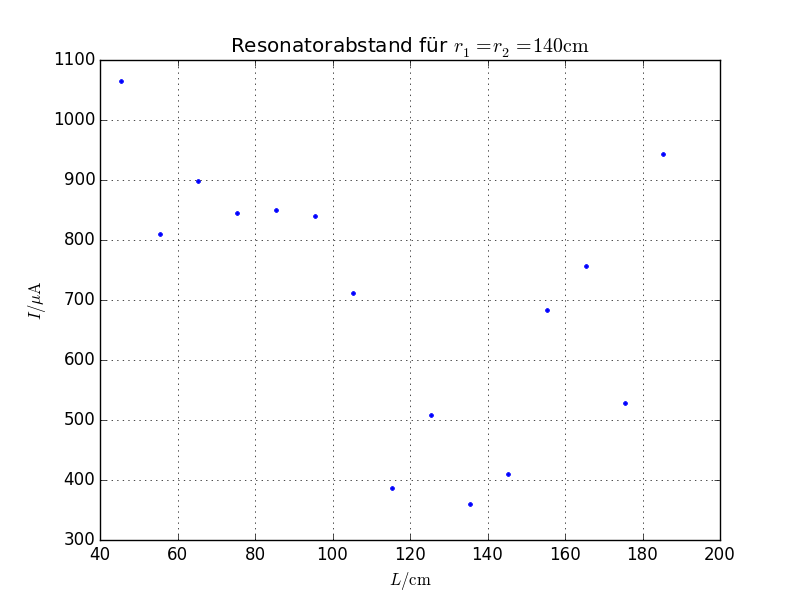
\includegraphics[width=0.5\textwidth]{stabil1.png}
	\caption{Resonatorabstand gegen Strom bei gleich gekrümmten Spiegeln}
	\label{fig:stabil1}
\end{figure}

\noindent Für Spiegel mit den Krümmungsradien \(r_1\neq r_2\) ist die Nullstelle der Funktion bei \(L=r_1\lor L=r_2\). Die Funktion wird für \(L=r_1+r_2\) gleich eins. Da \(r_1=\infty\) ist (planarer Spiegel), vereinfacht sich die Bedingung zu:

\begin{equation}
0\le1-\frac{1}{r_2}L<1
\end{equation}

\noindent was eine Geradengleichung mit negativer Steigung ist. Daraus folgt direkt, dass die Bedingung für das Intervall \(\mathbb{L}=(0,140]\).

\noindent Die gemessenen Werte sind Tabelle \ref{tab:t2} zu entnehmen.

\begin{table}[H]
	\begin{center}
		\begin{tabular}{c c}
			\toprule
			\(L+L_0\)/cm & \(I\)/\(\mu\)A \\
			\midrule
			55              &272          \\                                                                           
			65              &291        \\                                                                             
			75              &120      \\                                                                               
			85              &150    \\                                                                                 
			95              &60    \\                                                                                  
			105             &45 \\
			\bottomrule
		\end{tabular}
		\caption{Resonatorabstand für \(r_1=\infty\text{m}\), \(r_2=1,4\)cm}
		\label{tab:t2}
	\end{center}
\end{table}

\noindent Die graphische Darstellung von \(L\) gegen \(I\) ist in Abbildung \ref{fig:stabil2} gegeben.

\begin{figure}
	\centering
		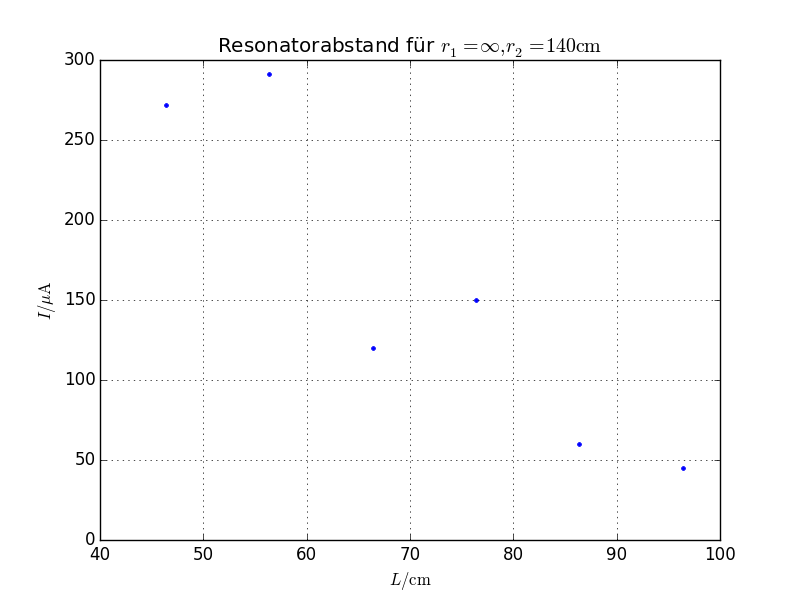
\includegraphics[width=0.5\textwidth]{stabil2.png}
	\caption{Resonatorabstand gegen Strom mit planarem Spiegel}
	\label{fig:stabil2}
\end{figure}

\subsection{TEM-Moden}
\subsection{Polarisation}
\subsection{Wellenlänge}

%%%%%%%%%%%%
%%% TABELLEN %%%
%%%%%%%%%%%%
\begin{table}[H]
	\begin{center}
		\begin{tabular}{c c}
			\toprule
			\(\phi\)/° & \(I\)/\(\mu\)A \\
			\midrule
			0       &24\\
			10      &67\\
			20      &114\\
			30      &216\\
			40      &261\\
			50      &384\\
			60      &499\\
			70      &381\\
			80      &448\\
			90      &393\\
			100     &316\\
			110     &284\\
			120     &207\\
			130     &114\\
			140     &64\\
			150     &22\\
			160     &2\\
			170     &3\\
			180     &24\\
			190     &65\\
			200     &124\\
			210     &213\\
			220     &331\\
			230     &403\\
			240     &453\\
			250     &510\\
			260     &493\\
			270     &460\\
			280     &371\\
			290     &284\\
			300     &200\\
			310     &127\\
			320     &60\\
			330     &23  \\                                                                                            
			340     &2      \\                                                                                         
			350     &3  	\\
			\bottomrule
		\end{tabular}
		\caption{Strom für verschiedene Winkel des Polfilters}
		\label{fig:t3}
	\end{center}
\end{table}

\begin{table}[H]
	\begin{center}
		\begin{tabular}{c c}
			\toprule
			\(d\)/mm & \(I\)/\(\mu\)A \\
			\midrule
			-15  &  0,46\\                                                                                            
			-14     &0,77  \\                                                                                          
			-13     &1,21    \\                                                                                        
			-12     &1,68      \\                                                                                      
			-11     &2,17        \\                                                                                    
			-10     &3,08          \\                                                                                  
			-9      &3,93             \\                                                                               
			-8      &4,56               \\                                                                             
			-7      &5,42                 \\
			-6      &5,80                   \\                                                                         
			-5      &6,61                     \\                                                                       
			-4      &5,88                       \\                                                                     
			-3      &6,01                         \\                                                                   
			-2      &5,33                           \\
			-1      &4,93\\
			0       &5,27\\
			1       &3,60\\
			2       &3,50\\
			3       &3,08\\
			4       &2,33\\
			5       &1,73\\
			6       &1,04\\
			7       &0,83\\
			8       &0,50\\
			9       &0,29\\
			\bottomrule
		\end{tabular}
		\caption{\(\text{TEM}_{00} Grundmode\)}
		\label{fig:t4}
	\end{center}
\end{table}

\begin{table}[H]
	\begin{center}
		\begin{tabular}{c c}
			\toprule
			\(d\)/mm & \(I\)/\(\mu\)A \\
			\midrule
			-24     &0\\
			-22     &0\\
			-20     &0,03\\
			-18     &0,10\\
			-16     &0,21\\
			-14     &0,35\\
			-12     &0,60\\
			-10     &0,77\\
			-8      &0,57\\
			-6      &0,23\\
			-4      &0,02\\
			-2      &0,04\\
			0       &0,17\\
			2       &0,24\\
			4       &0,38\\
			6       &0,31\\
			8       &0,26\\
			10     & 0,16\\
			12      &0,09\\
			14      &0,04\\
			\bottomrule
		\end{tabular}
		\caption{\(\text{TEM}_{10} Mode\)}
		\label{fig:t5}
	\end{center}
\end{table}